\chapter{Results}
\label{results}
All chapters must start on a right hand page!

\section{My first great results involves theorems, lemmas and examples}
All results must be given a continuous numbering for cross reference and future citations. This template is set up with a suitable numbering and correct typesetting for the most used theoremstyles in the \texttt{uiotools}-file; see this file if you want customize or make a new environment. 

\begin{example}
    This is an example.
\end{example}

\begin{definition}
    This is a definition.
\end{definition}

\begin{theorem}
    This is a theorem.
\end{theorem}

\begin{proof}
    This is a proof.
\end{proof}

\begin{remark}
 This is a remark.    
\end{remark}



\section{My second great result involves figures and tables}
Figures and tables are important, and they must be included with floats, which makes them pop up wherever \LaTeX wants them to. This can seem unfamiliar for a novice \LaTeX user, and requires two things. First, you must include a caption below your figure or above your table containing a short explanation. Secondly, you must comment on your figure or table in your text. This can be done by adding a label underneath the caption in the environment, followed by adding a suitable cross reference in the text. 

It is wise to use labels that are easy to recall, preferably systematic with a prefix followed by a description, f.ex. fig:oneball. Using draft mode and the package {\texttt {showkeys}} the labels (and citekeys) are displayed above the text or in the margins, which is very convenient when you work with a large document. This is turned off by adding the option \enquote{final} to the documentclass.

To produce the cross reference, use the command \texttt{\textbackslash cref} (\cref{fig:twoballs}) to call upon the label and an automatic description of the object. If you want a description of the placement of the environment in your cross reference, use \texttt{\textbackslash vref} (\vref{fig:twoballs}), which will add the location or page number if the figure shows up on a page further away. Read more about \hyperlink{https://latex-tutorial.com/advanced-latex-cross-references/}{cross references} in this link \cite{CREF}.

Note that it is possible to tweak the placement of a float using the float specifier option [htbp], where h stands for here, t for top, b for bottom and p for page, but please don't spend time doing that before the week before the due date. Sometimes it is better to include just a little text or move the float in the code.

\subsection{Figures}
Adding a floating environment and presenting a figure, graph or picture can be done in several different ways. The two most common ways are to use \texttt{\textbackslash input}, see \vref{fig:oneball}, or \texttt{\textbackslash includegrapics}, see \vref{fig:twoballs}. 
% Tikzfigure with \input:
\begin{figure}
    \centering
    \input{figures/ball}
    \caption[One ball (to appear in LOF)]{This is a figure of one ball, and the caption goes underneath the figure. This could be a complete description of the figure in several sentences. A shorter caption should be made for List of Figures.}
    \label{fig:oneball}
\end{figure}

Note that \vref{fig:twoballs} has a long caption, which is not suitable for the List of Figures at the beginning of the thesis. A shorter caption, more or less a caption-title, should be added as an option.

You can adjust the size of the graphic as you wish by adding options for height and width, crop it and more, but make sure that you have a figure with sufficient resolution, see \vref{fig:twoballs}.

% Includegraphics
\begin{figure}[h]
    \centering
    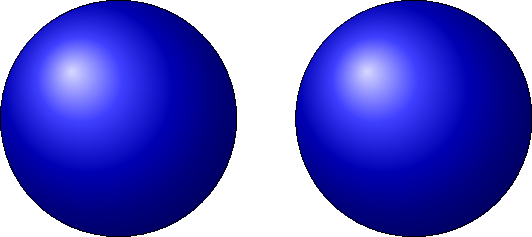
\includegraphics[width=\textwidth]{figures/balls.pdf}
    \caption[Two balls]{Two balls.}
    \label{fig:twoballs}
\end{figure}

When you write your thesis, you sometimes just know that you need some text or a figure, but you have not made it yet. Then you can include a todo-note and a missing figure, see \vref{fig:missing}. \todo{I must write a paragraph about this here.}

% Todonotes:
\begin{figure}
    \centering
    \missingfigure{Three balls.}
    \caption[Three balls]{I have to make a figure with three balls before I forget how!}
    \label{fig:missing}
\end{figure}

\begin{remark}
    There are so many floats in a row here, that \LaTeX\; struggles to place them, but resist the temptation to tweak the placement before the final touch!
\end{remark}

\subsection{Tables}
There is a lot to say about tables, but the main point is that we use the package \texttt{booktabs} to create tables with as few lines and good spacing as possible. The first row is usually descriptive and in a different font (bold, textsf etc.). If you need huge or complicated tables with multilines or -columns, try to instruct AI to create the \LaTeX-code for this or copy from an online instruction manual; this is not considered plagiarism. Note that there are solutions for tables over multiple pages and tables that extend to the margins, hence need to be rotated $90$ degrees.

The examples that follow here, show typical tables with caption above the table - but please notice the important information in the tables as well.

% Booktabs:
\begin{table}
    \centering
       \caption[Colons (to appear in LOT)]{Caption above tables. Proper colon usage. Alternative for List of Tables.}
           \label{tab:colon}
    \begin{tabular}{@{}ll@{}}
        \toprule
        \textsf{Correct}               & \textsf{Incorrect}      \\
        \midrule
        \( \varphi \colon X \to Y \)   & \( \varphi : X \to Y \) \\[0.5ex]
        \( \varphi(x) \coloneqq x^2 \) & \( \varphi(x) := x^2 \) \\
        \bottomrule
    \end{tabular}
\end{table}

\begin{table}
    \centering
    \caption[Arrows]{Proper arrow usage.}
    \begin{tabular}{@{}ll@{}}
        \toprule
        \textsf{Correct}     & \textsf{Incorrect}         \\
        \midrule
        \( A \implies B \)   & \( A \Rightarrow B \)      \\
        \( A \impliedby B \) & \( A \Leftarrow B \)       \\
        \( A \iff B \)       & \( A \Leftrightarrow B \)  \\
        \bottomrule
    \end{tabular}
 
\end{table}

\begin{table}
      \caption[Quotation marks]
    {Proper quotation mark usage.
    The \texttt{\textbackslash enquote} command chooses the correct
    quotation marks for the specified language. Moreover, \texttt{\textbackslash resizebox} has been used to control table width.}
    \centering
     \resizebox{\linewidth}{!} {
      \begin{tabular}{@{}*{2}{p{0.5\textwidth}}@{}}
           \toprule
        \textsf{Correct} &  \textsf{Incorrect}
        \\
        \midrule
        \enquote{This is an \enquote{inner quote} inside an outer quote} (Controlled by \enquote{babel}.)
        &
        'This is an "inner quote" inside an outer quote'
        \\
        \bottomrule
    \end{tabular}
    }
    \label{tab14}
\end{table}

% Tablefootnote and multirow:
\begin{table}
   \caption[Dashes]{Proper dash usage. Minus is not minus unless it's in math mode. Intervals are longer than expected. It is now easy to tell that Birch and Swinnerton-Dyer are two people, but I don't know why the footnote lands on the wrong page.}
    \centering
    \begin{tabular}{@{}ll@{}}
        \toprule
        \textsf{Correct}
        & 
        \textsf{Incorrect}
        \\
        \midrule
        \( -1 \) 
        & 
        -1
        \\[0.3ex]
        1--10
        &
        1-10
        \\[0.3ex]
        Birch--Swinnerton-Dyer conjecture
        &
        Birch-Swinnerton-Dyer conjecture
        \\[0.3ex]
        The ball \dash which is blue \dash is round.
        &
        \multirow{ 2}{*}{The ball - which is blue - is round.}
        \\[0.3ex]
        The ball---which is blue---is round. 
        &
        \\
        \bottomrule
    \end{tabular}
  
\end{table}


